\documentclass{article}
\usepackage[a4paper, total={7in, 9.5in}]{geometry}
\usepackage{amsmath,amsfonts,amsthm,amssymb,graphicx,float, setspace, bm}
\usepackage[utf8]{inputenc}
\usepackage{float}
\usepackage{titlesec}
\usepackage{setspace}
\usepackage{geometry}
\usepackage[style=numeric]{biblatex}
\usepackage[autostyle=true]{csquotes}
\usepackage{breqn}
\usepackage{subfig}
\usepackage[bottom]{footmisc}
\usepackage{adjustbox}
\usepackage{lipsum}
\usepackage{hyperref}
\usepackage[ruled,vlined]{algorithm2e}
\hypersetup{
    colorlinks=true,
    urlcolor=magenta
}
\usepackage[table,x11names]{xcolor}

\usepackage{xltabular}
\usepackage{multirow}
\usepackage{booktabs}


\renewcommand{\baselinestretch}{1.5} 
\setlength\parindent{0pt}
%----------------------------------------------------------------------------------------
%	START
%----------------------------------------------------------------------------------------

\newcommand{\horrule}[1]{\rule{\linewidth}{#1}}

\title{ \normalfont \normalsize 
\huge CPSC 532W - Homework 4}
\date{}
\author{Xiaoxuan Liang - 48131163}
\def\cond{\; | \;}

\begin{document}

\maketitle

Public GitHub repo: https://github.com/Xiaoxuan1121/CPSC532W/tree/main/a4
\begin{enumerate}
\item Code snippets:

\begin{figure}[!ht]
	\centering
	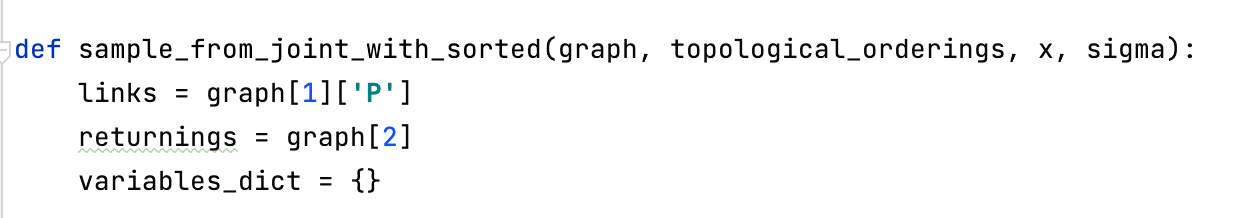
\includegraphics[scale=0.5]{../figs/graph_evaluator_1}
	\caption{code for graph evaluator part I}
\end{figure}

\begin{figure}[!ht]
	\centering
	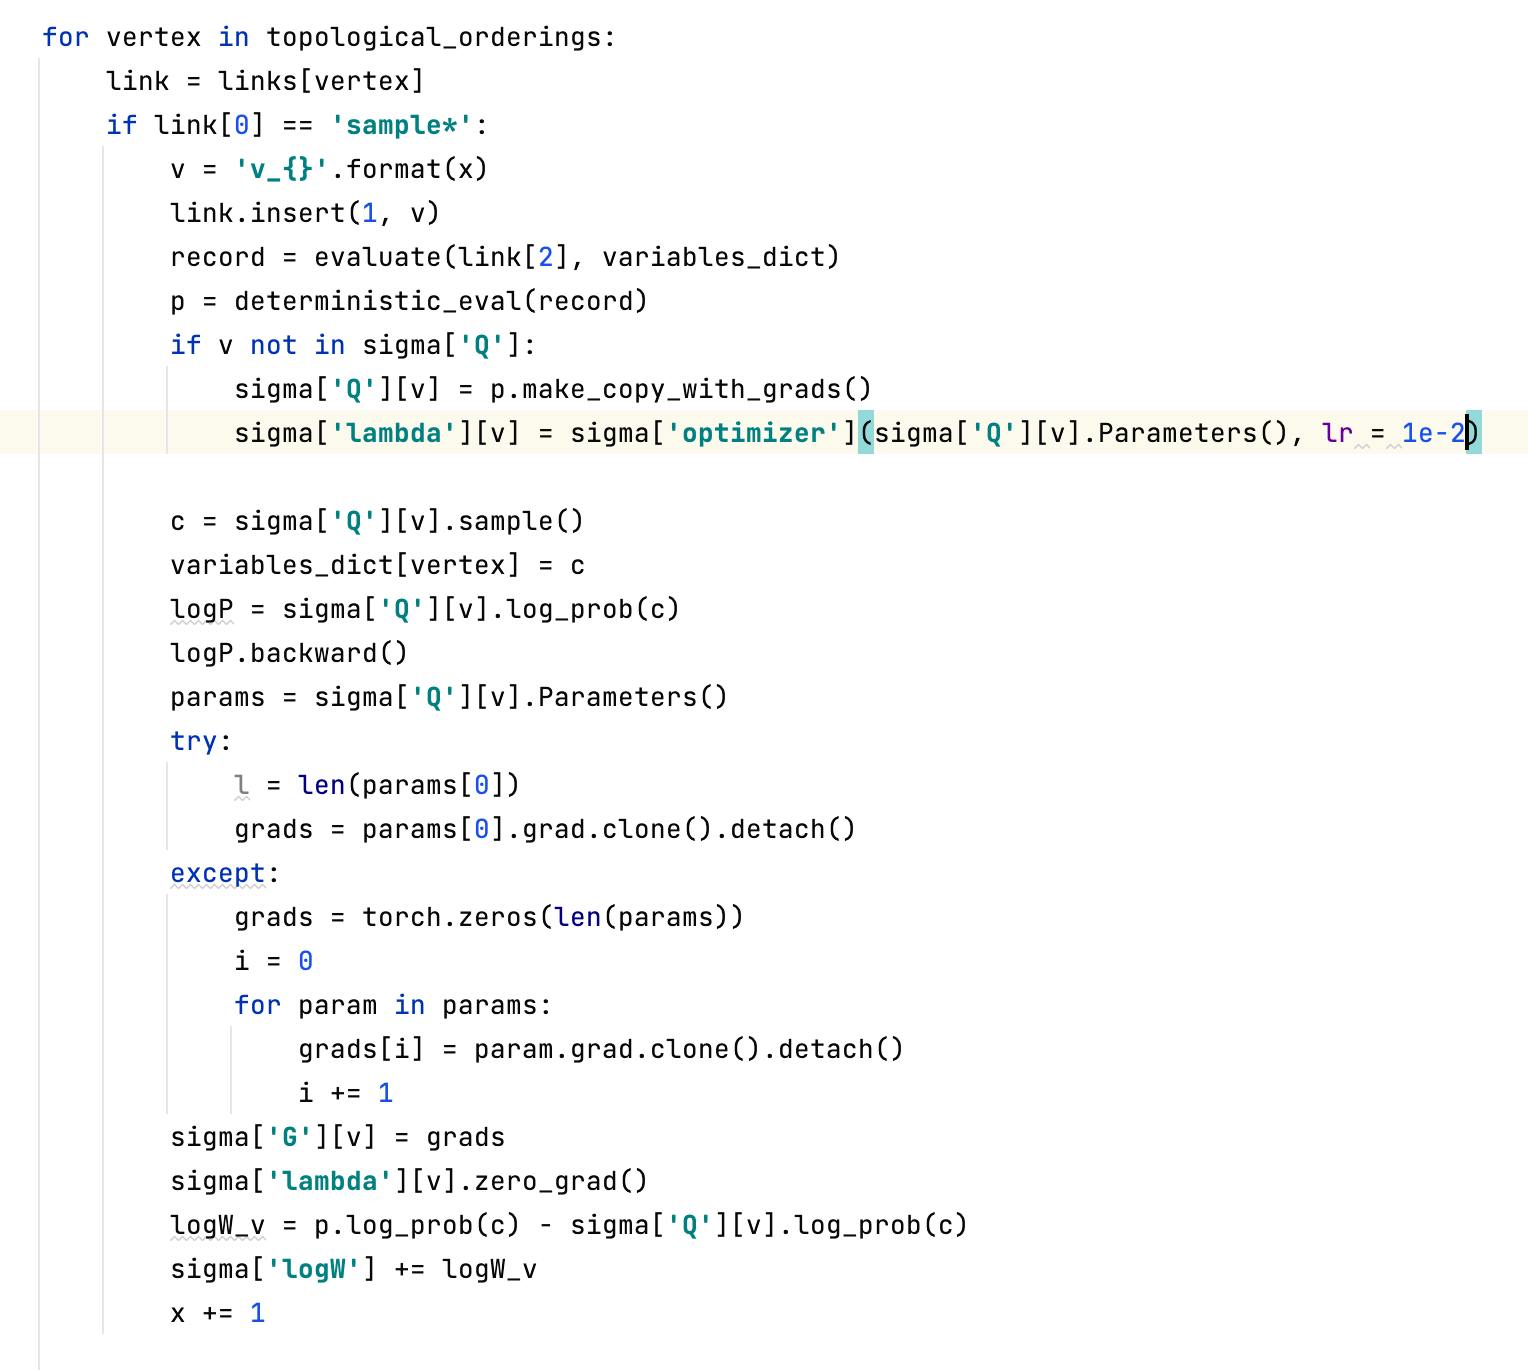
\includegraphics[scale=0.5]{../figs/graph_evaluator_2}
	\caption{code for graph evaluator part II}
\end{figure}

\newpage
\begin{figure}[!ht]
	\centering
	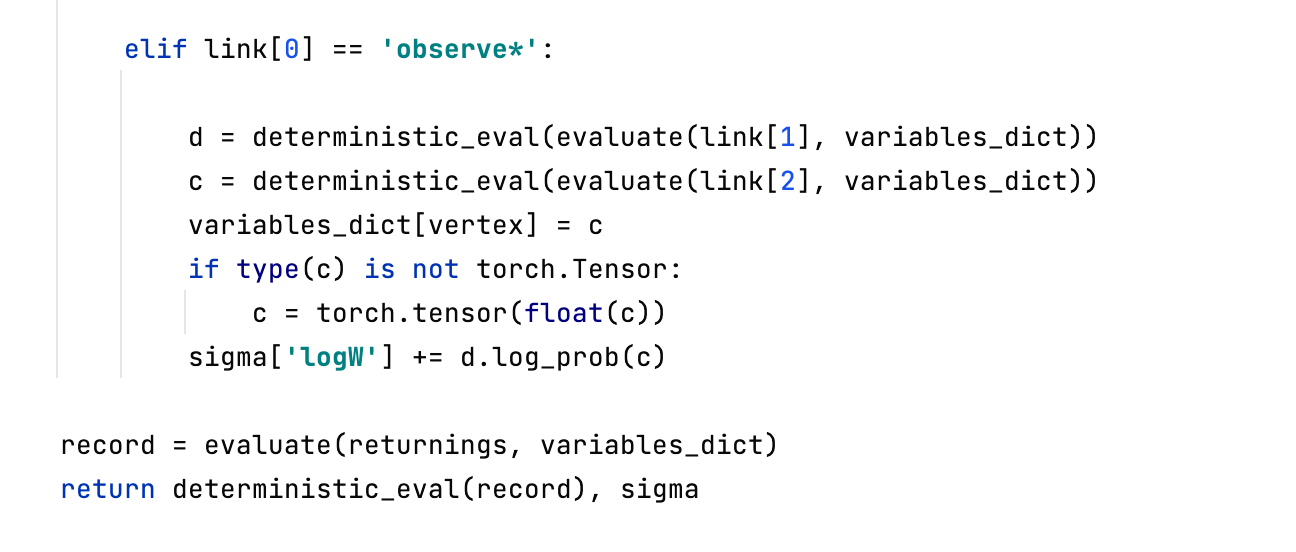
\includegraphics[scale=0.5]{../figs/graph_evaluator_3}
	\caption{code for graph evaluator part III}
\end{figure}

\begin{figure}[!ht]
	\centering
	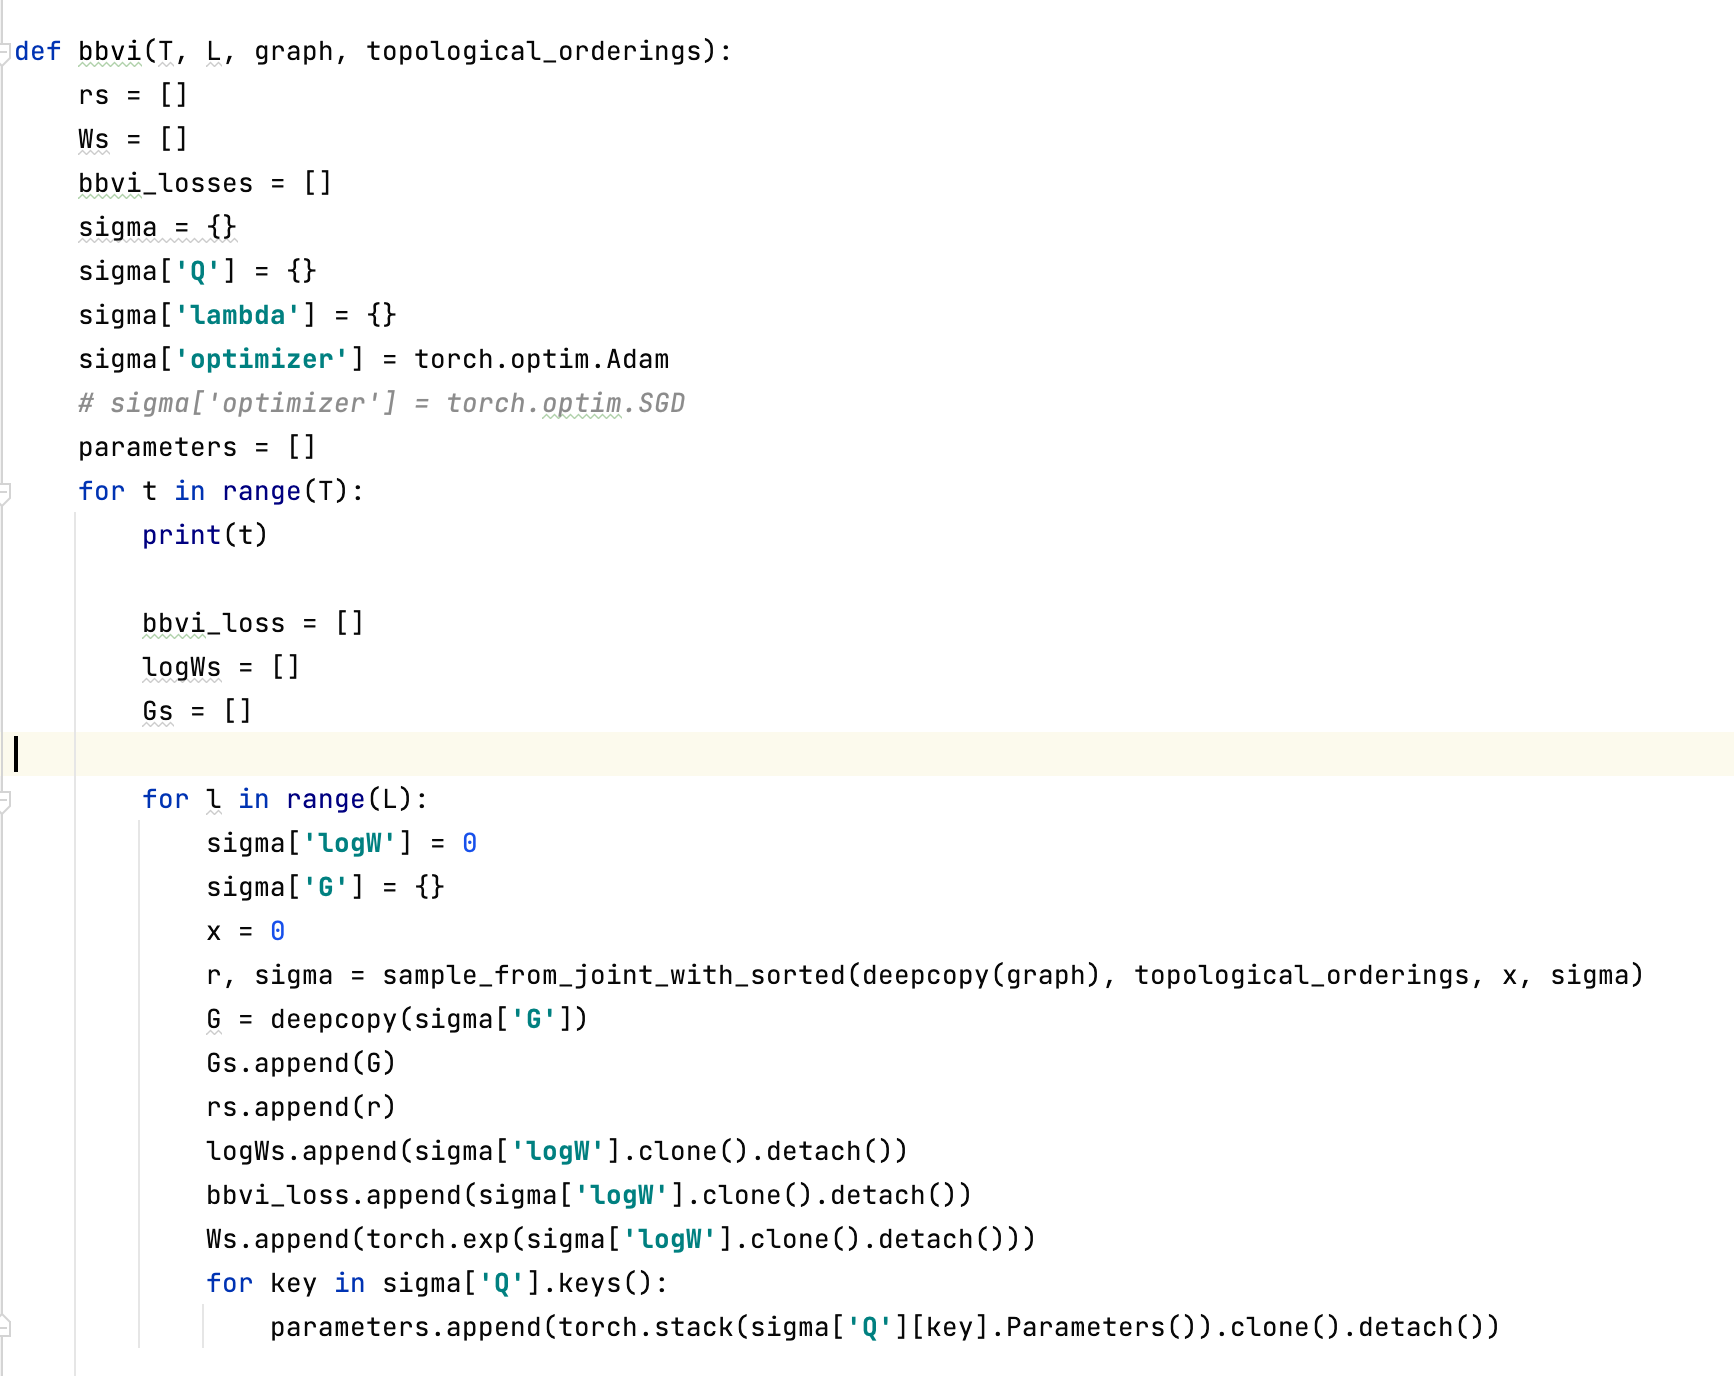
\includegraphics[scale=0.5]{../figs/bbvi_1}
	\caption{code for BBVI part I}
\end{figure}

\newpage
\begin{figure}[!ht]
	\centering
	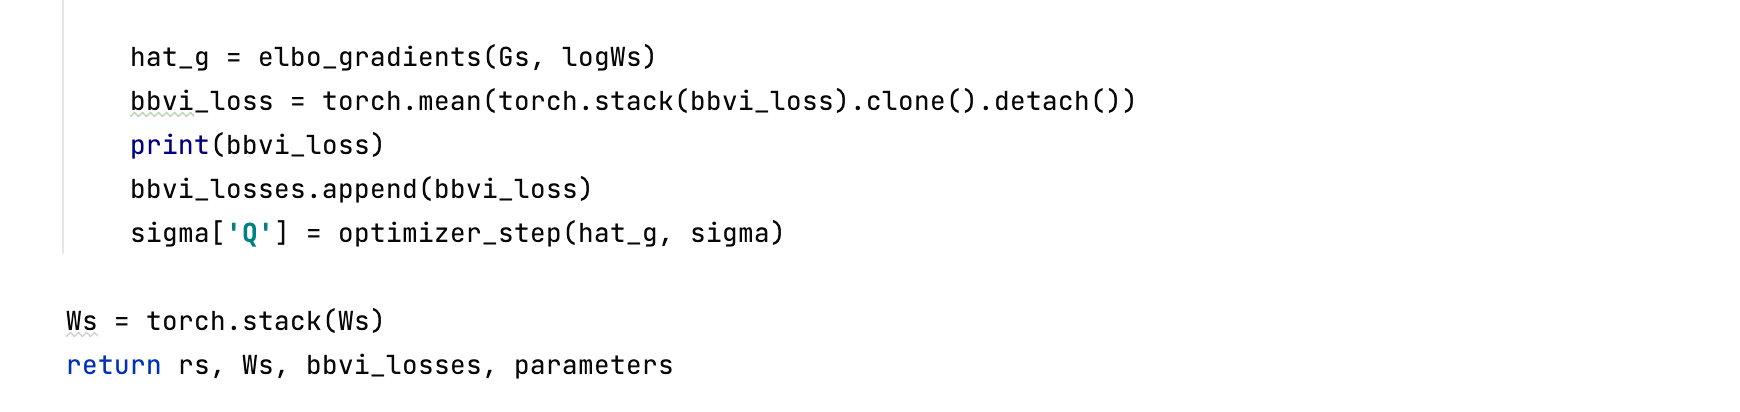
\includegraphics[scale=0.5]{../figs/bbvi_2}
	\caption{code for BBVI part II}
\end{figure}

\begin{figure}[!ht]
	\centering
	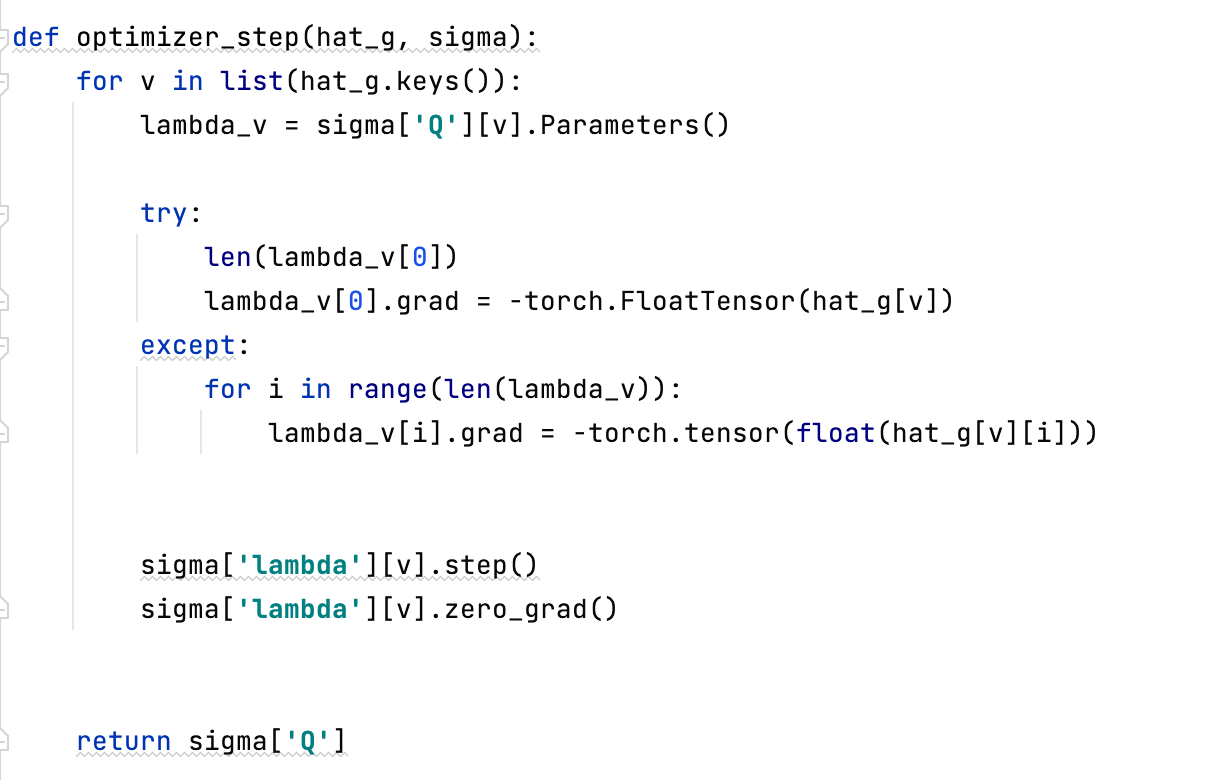
\includegraphics[scale=0.5]{../figs/bbvi_3}
	\caption{code for BBVI part III}
\end{figure}

\newpage
\begin{figure}[!ht]
	\centering
	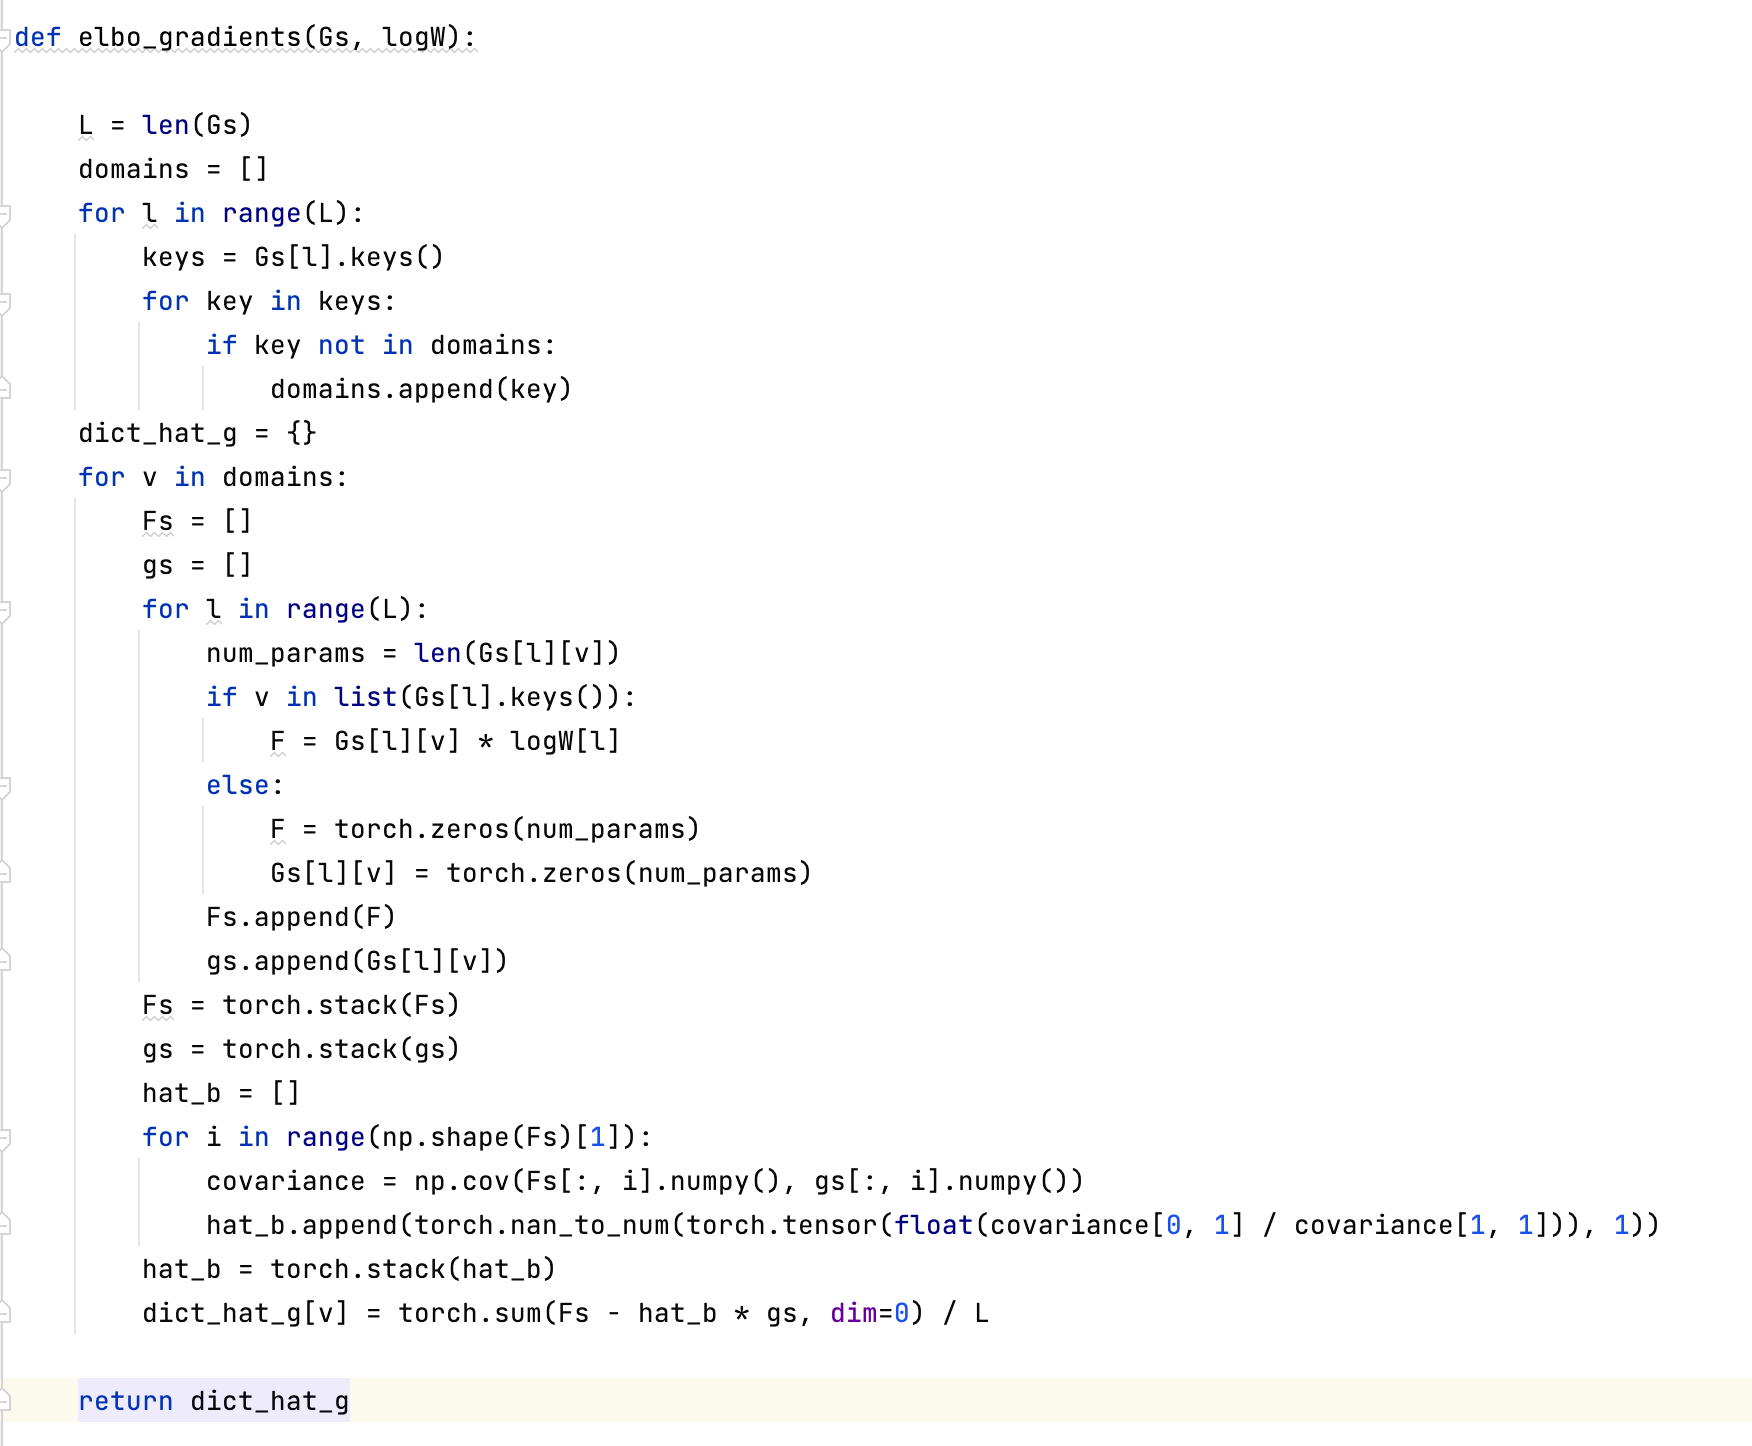
\includegraphics[scale=0.5]{../figs/bbvi_4}
	\caption{code for BBVI part IV}
\end{figure}

\newpage
\item Program 1: \\
The posterior expected value of mu is $7.2577$.  \\
The variational distribution of $\mu$ is a Normal distribution with mean $7.25$ and $0.3998$.

\begin{figure}[!ht]
	\centering
	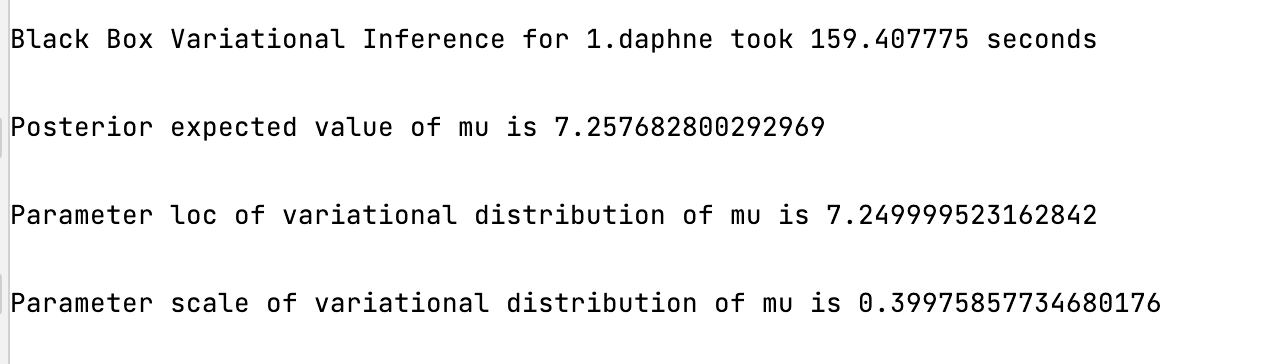
\includegraphics[scale=0.5]{../figs/1_daphne_results}
\end{figure}

\begin{figure}[!ht]
	\centering
	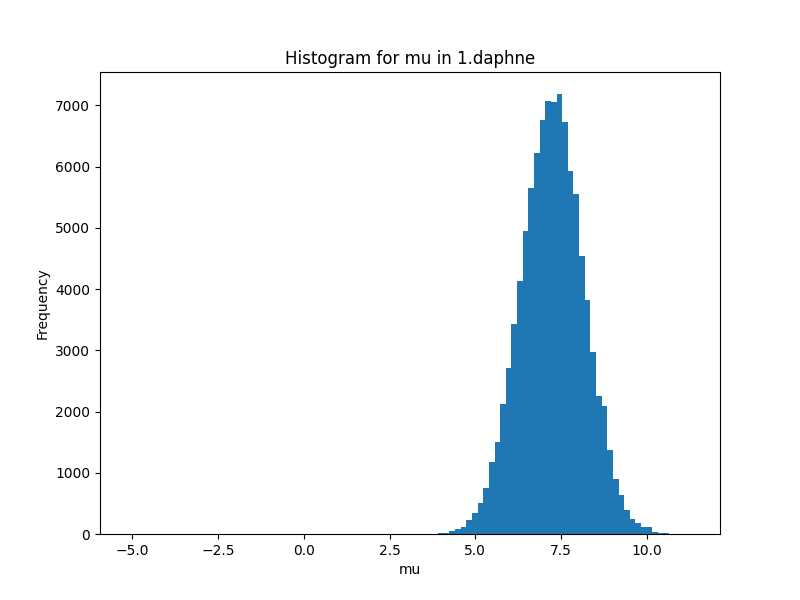
\includegraphics[scale=0.5]{../figs/1_daphne_histogram}
	\caption{Posterior distribution for mu for 1.daphne using Black Box Variational Inference}
\end{figure}

\begin{figure}[!ht]
	\centering
	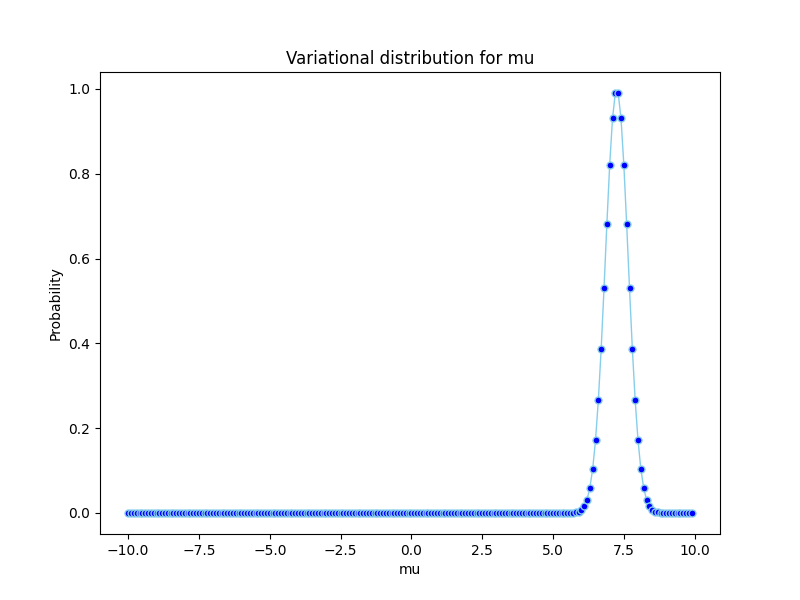
\includegraphics[scale=0.5]{../figs/1_daphne_pdf}
	\caption{Variational distribution for mu for 1.daphne using Black Box Variational Inference}
\end{figure}

\begin{figure}[!ht]
	\centering
	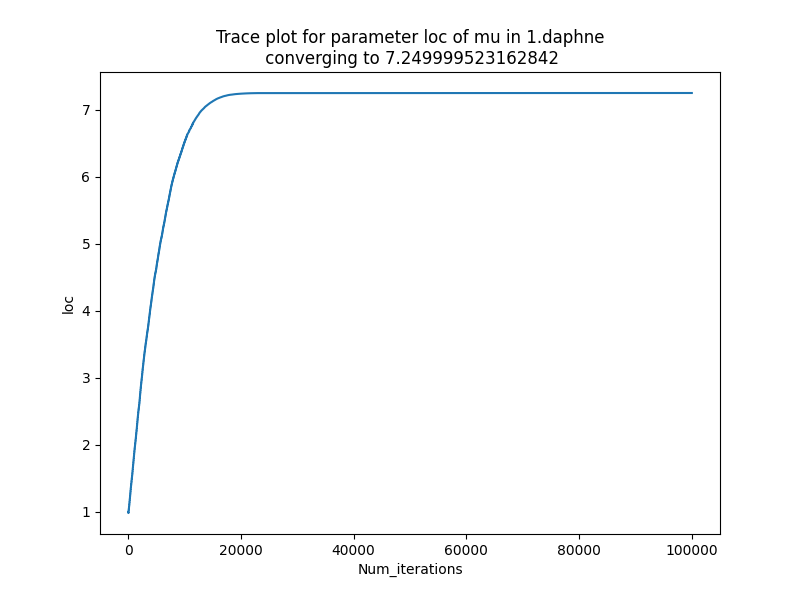
\includegraphics[scale=0.5]{../figs/1_daphne_loc_trace}
	\caption{Trace plot for parameter loc of mu in 1.daphne}
\end{figure}

\newpage
\begin{figure}[!ht]
	\centering
	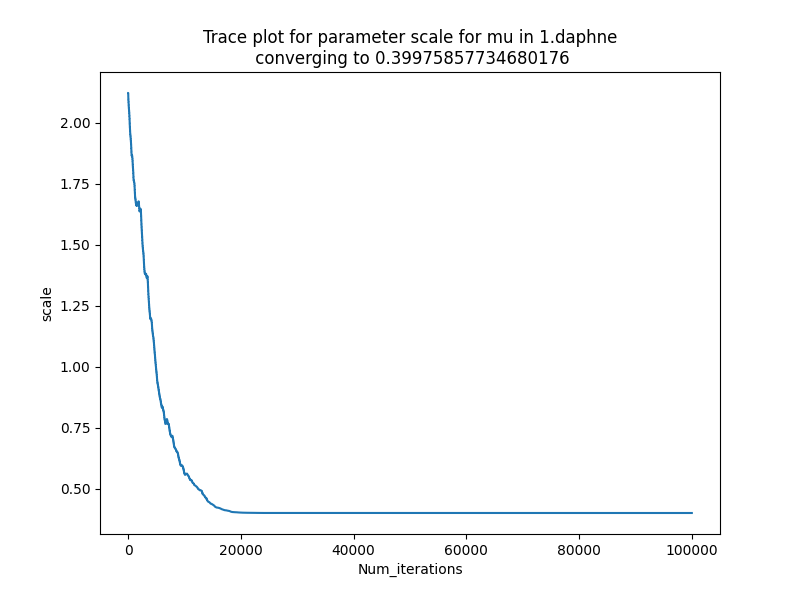
\includegraphics[scale=0.5]{../figs/1_daphne_scale_trace}
	\caption{Trace plot for parameter scale of mu in 1.daphne}
\end{figure}

\begin{figure}[!ht]
	\centering
	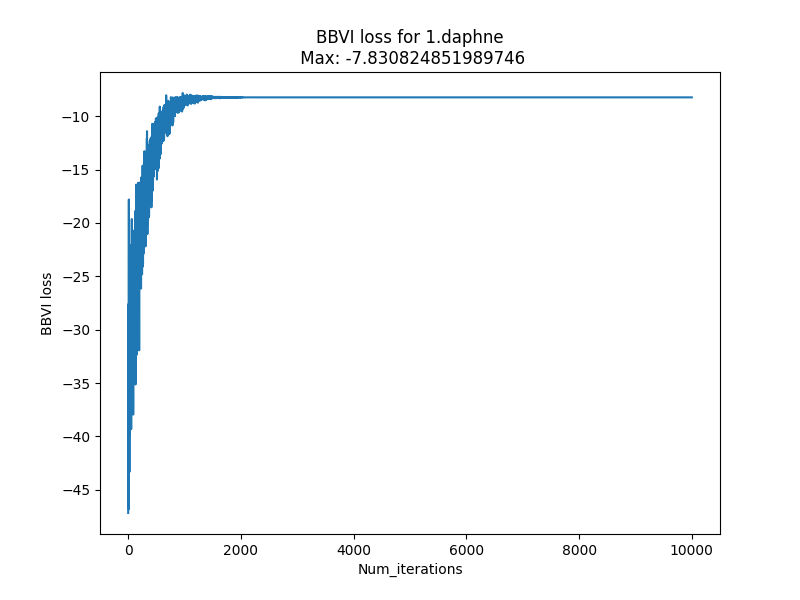
\includegraphics[scale=0.5]{../figs/1_daphne_ELBO}
	\caption{ELBO for 1.daphne}
\end{figure}

\newpage
\item Program 2:

\begin{figure}[!ht]
	\centering
	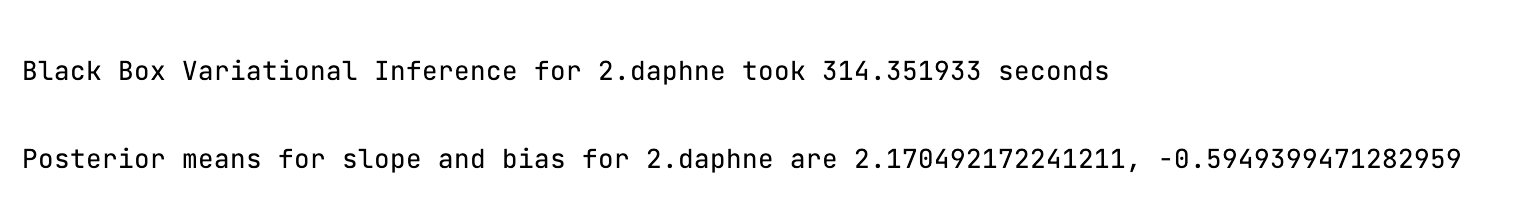
\includegraphics[scale=0.5]{../figs/2_daphne_results}
\end{figure}


\begin{figure}[!htp] 
    \centering
    \subfloat[Samples from the posterior for slope]{%
        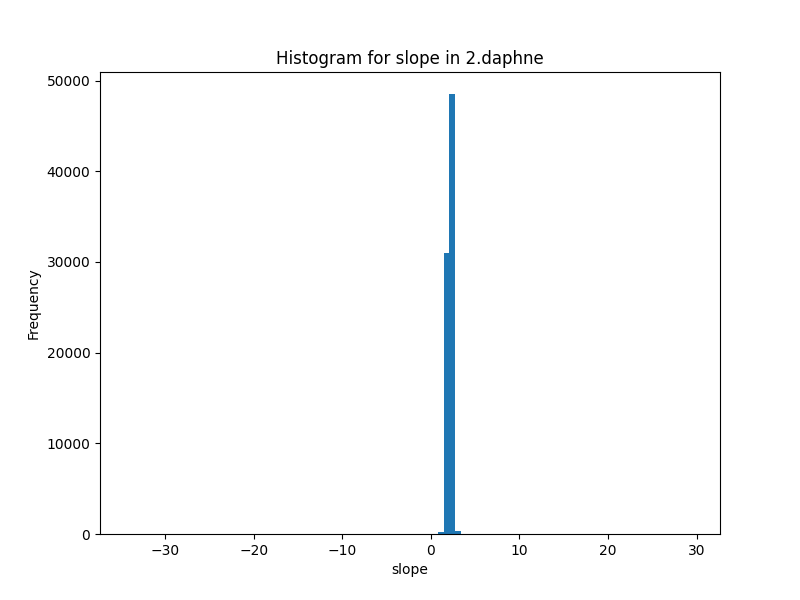
\includegraphics[width=0.5\textwidth]{../figs/2_daphne_slope_histogram}%
        \label{fig:a}%
        }%
    \hfill%
    \subfloat[Samples from the posterior for bias]{%
        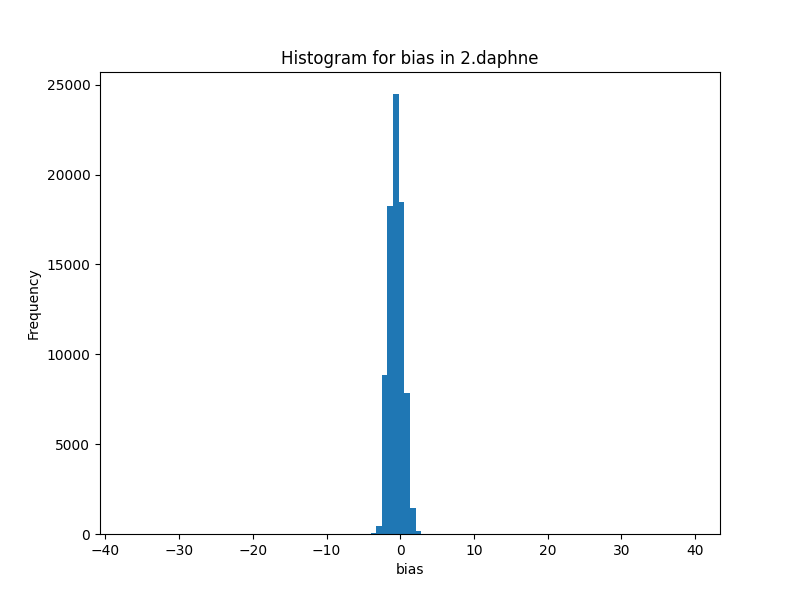
\includegraphics[width=0.5\textwidth]{../figs/2_daphne_bias_histogram}%%
        \label{fig:b}%
        }%
        \caption{Posterior distribution for slope and bias for 2.daphne using Black Box Variational Inference}
\end{figure}

\begin{figure}[!ht]
	\centering
	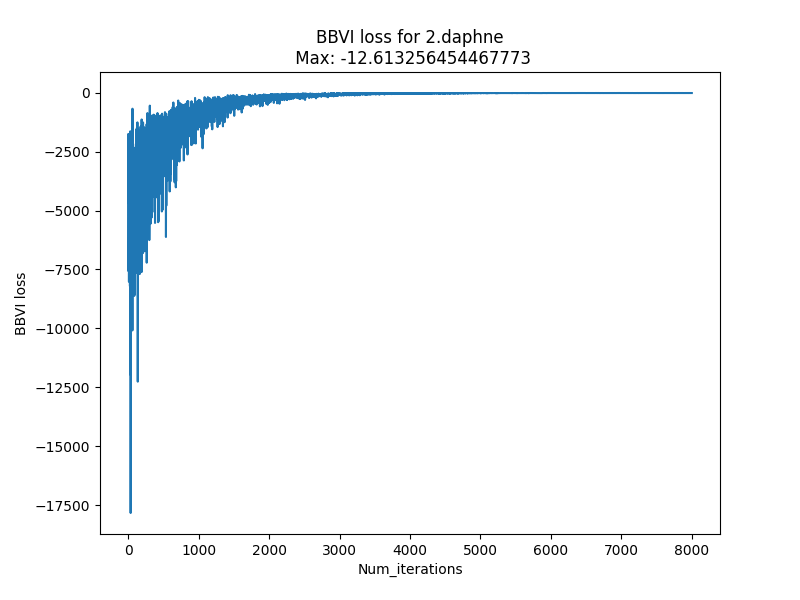
\includegraphics[scale=0.5]{../figs/2_daphne_ELBO}
	\caption{ELBO for 2.daphne}
\end{figure}

\newpage
\item  Program 3:

\begin{figure}[!ht]
	\centering
	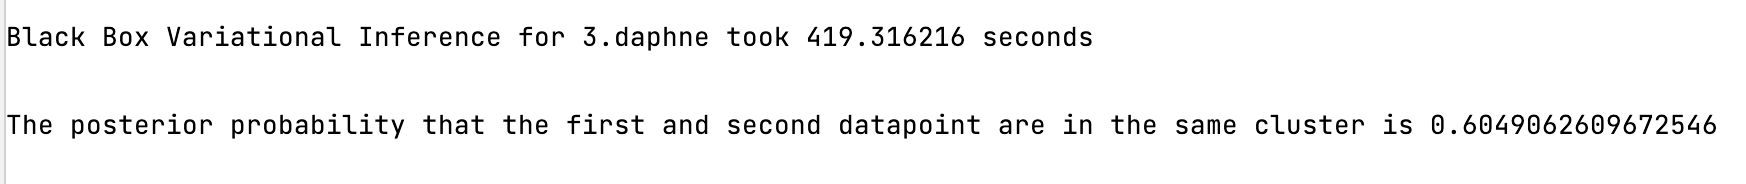
\includegraphics[scale=0.5]{../figs/3_daphne_results}
\end{figure}


\begin{figure}[!ht]
	\centering
	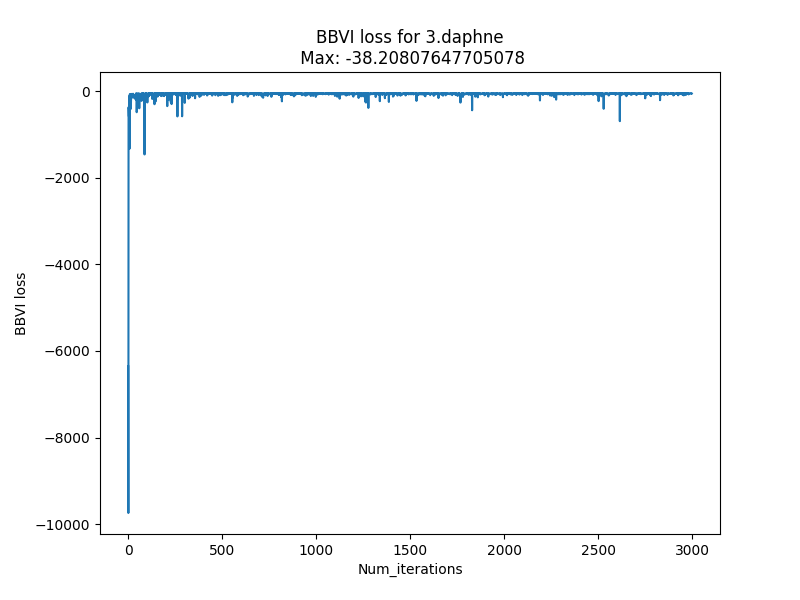
\includegraphics[scale=0.5]{../figs/3_daphne_ELBO}
\end{figure}

The mode-seeking behaviour of VI on models would fall into different modes every time when repeating running the code with internal symmetries.  Internal symmetries indicates the label switching problems, such that the class would be labelled (latent variables) by different notation since the labels are permuted randomly each time. This always happens in the mixture models,  however,  the model density is not changing even the labels are keeping switching among the classes. This might result in the inference analysis fall off sometimes and it will be back on the track after that, which canbe seen from the ELBO plot that the BBVI loss could suddenly drop down to a value and it will bounce back later.


\item  Program 4:

\begin{figure}[!ht]
	\centering
	
\includegraphics[scale=0.5]{../figs/4_daphne_results}
\end{figure}

\begin{figure}[!ht]
	\centering
	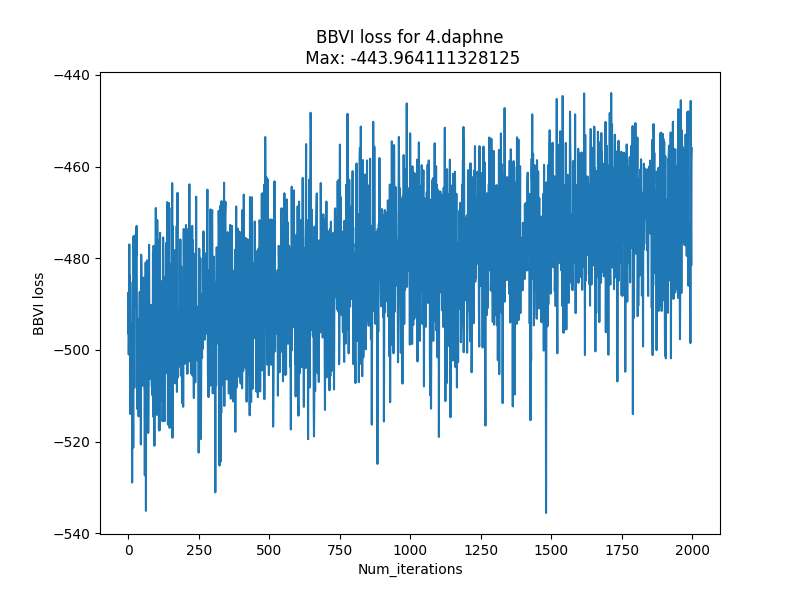
\includegraphics[scale=0.5]{../figs/4_daphne_ELBO}
	\caption{ELBO for 4.daphne}
\end{figure}

\begin{figure}[!htp] 
    \centering
    \subfloat[Samples from the posterior for W0]{%
        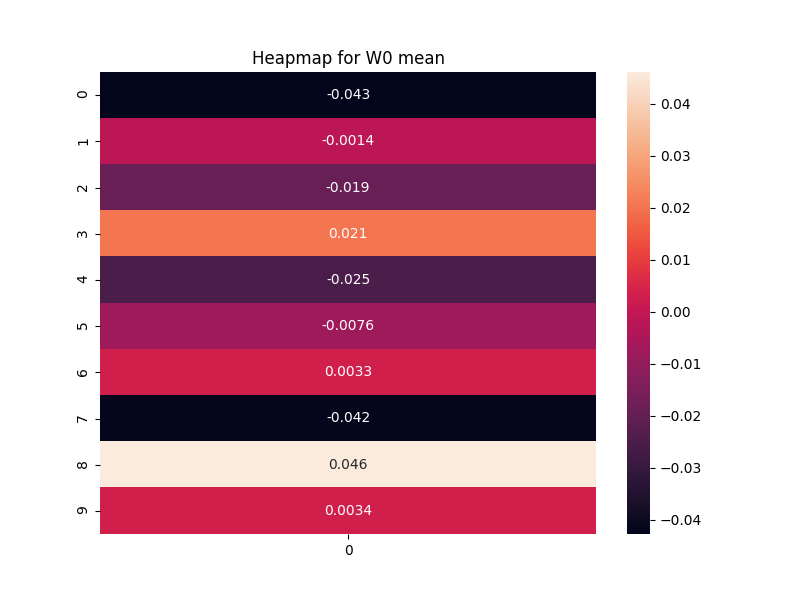
\includegraphics[width=0.5\textwidth]{../figs/4_daphne_w0_mean_heatmap.png}%
        \label{fig:a}%
        }%
    \hfill%
    \subfloat[Samples from the posterior for W0]{%
        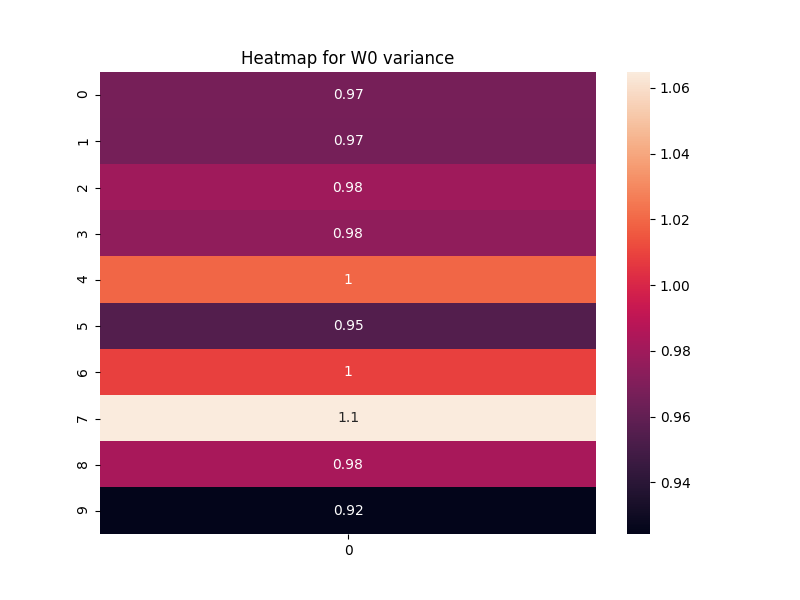
\includegraphics[width=0.5\textwidth]{../figs/4_daphne_w0_variance_heatmap.png}%%
        \label{fig:b}%
        }%
        \caption{Posterior distribution for slope and bias for 4.daphne using Black Box Variational Inference}
\end{figure}

\begin{figure}[!htp] 
    \centering
    \subfloat[Samples from the posterior for b0]{%
        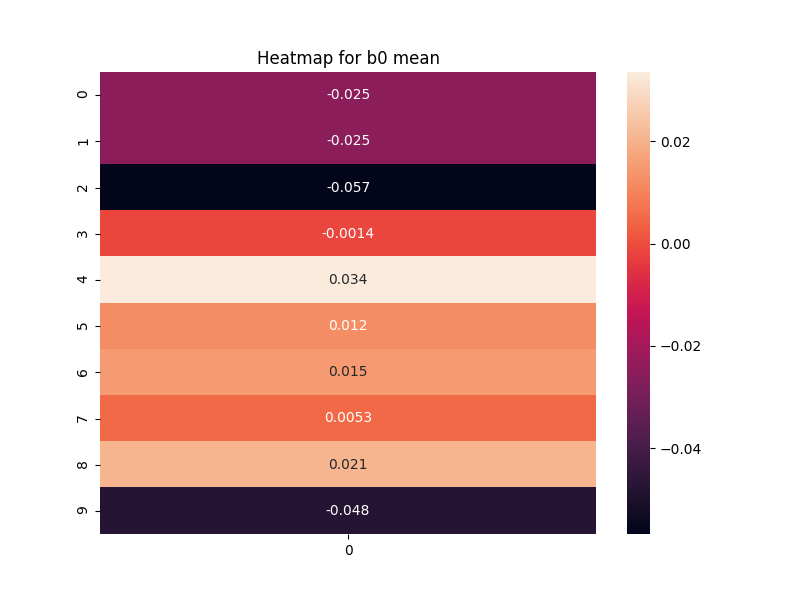
\includegraphics[width=0.5\textwidth]{../figs/4_daphne_b0_mean_heatmap.png}%
        \label{fig:a}%
        }%
    \hfill%
    \subfloat[Samples from the posterior for b0]{%
        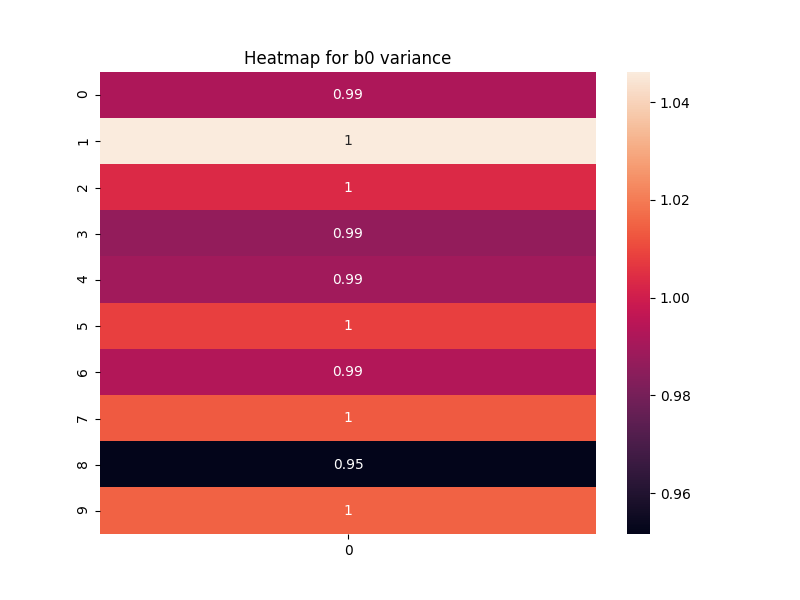
\includegraphics[width=0.5\textwidth]{../figs/4_daphne_b0_variance_heatmap.png}%%
        \label{fig:b}%
        }%
        \caption{Posterior distribution for slope and bias for 4.daphne using Black Box Variational Inference}
\end{figure}

\begin{figure}[!htp] 
    \centering
    \subfloat[Samples from the posterior for W1]{%
        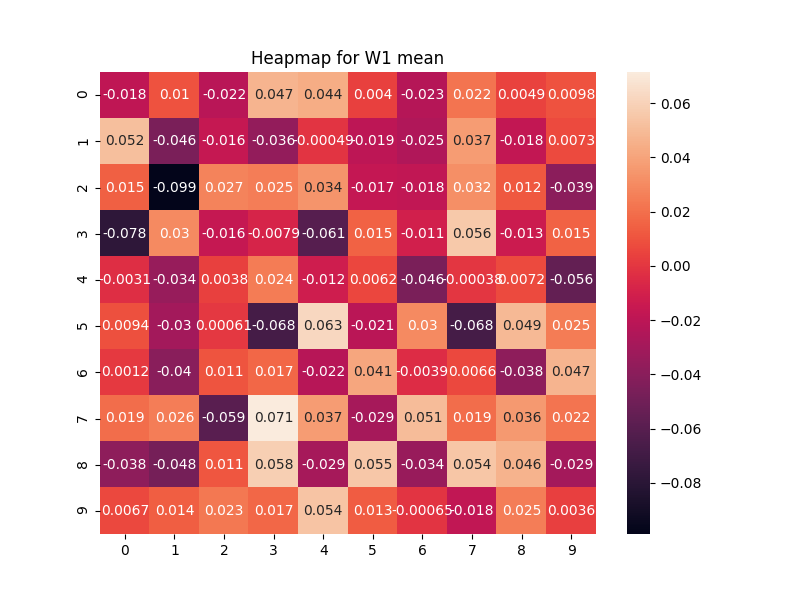
\includegraphics[width=0.5\textwidth]{../figs/4_daphne_w1_mean_heatmap.png}%
        \label{fig:a}%
        }%
    \hfill%
    \subfloat[Samples from the posterior for W1]{%
        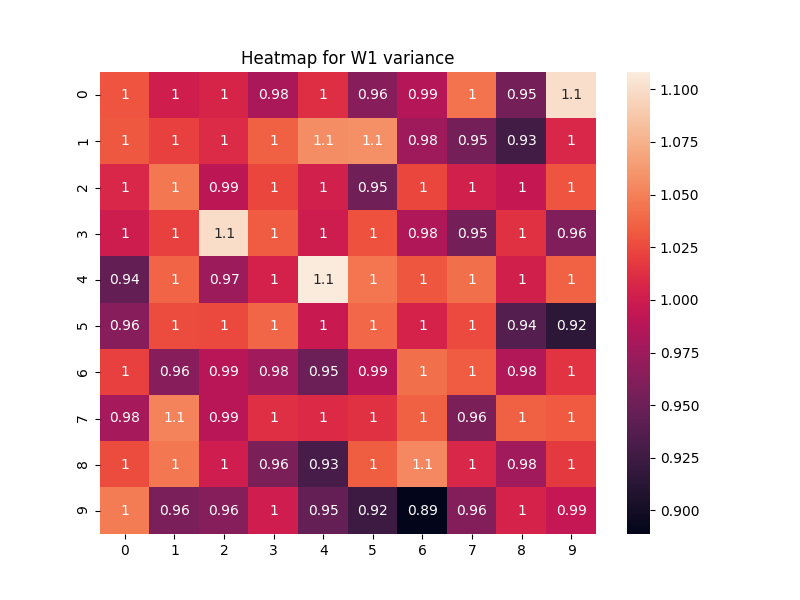
\includegraphics[width=0.5\textwidth]{../figs/4_daphne_w1_variance_heatmap.png}%%
        \label{fig:b}%
        }%
        \caption{Posterior distribution for slope and bias for 4.daphne using Black Box Variational Inference}
\end{figure}

\begin{figure}[!htp] 
    \centering
    \subfloat[Samples from the posterior for b1]{%
        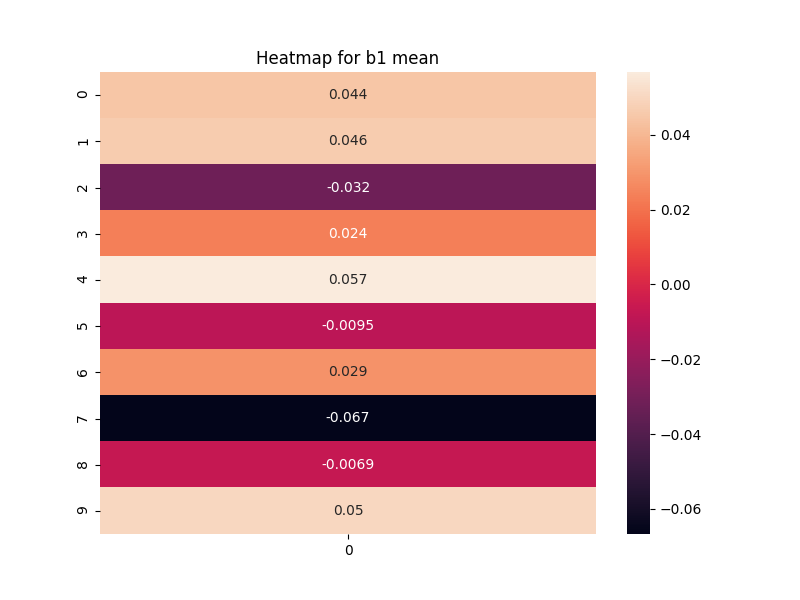
\includegraphics[width=0.5\textwidth]{../figs/4_daphne_b1_mean_heatmap.png}%
        \label{fig:a}%
        }%
    \hfill%
    \subfloat[Samples from the posterior for b1]{%
        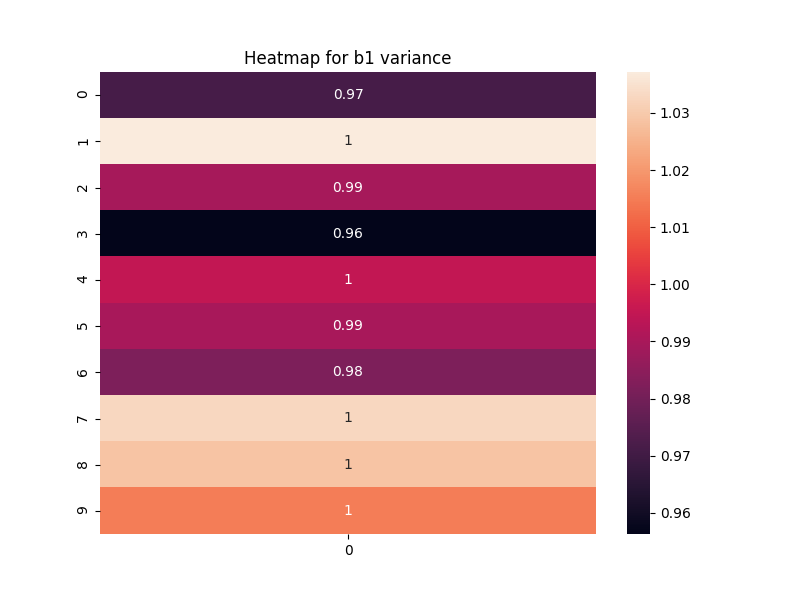
\includegraphics[width=0.5\textwidth]{../figs/4_daphne_b1_variance_heatmap.png}%%
        \label{fig:b}%
        }%
        \caption{Posterior distribution for slope and bias for 4.daphne using Black Box Variational Inference}
\end{figure}

\newpage
Mean-field black-box variational inference can be more widely used since we start from sampling from a prior distribution and keep updating the estimated parameters in posterior distribution by optimizing the evidence lower bound (ELBO),  while parameter estimation via gradient descent keeps computing gradient so the function has to be differentiable, and more preferably,  gradient is easy to obtain and compute with.  Therefore,  mean-field black-box variational inference can be applied to more complicated questions and a more generalizable method to use. 


\item Program 5:\\
To make the program run, we propose the distribution for continuous-uniform distribution with Gamma distribution with parameters $2$ and $m$ sampled from its distribution as the domain of Gamma distribution is the positive real line, satisfying the variance represented by m in normal distribution is always positive.  The parameters of learned variational distribution are fluctuating,  and we choose the last updated parameters in the gamma distribution as the final decision.\\
The learned variational distribution for s is Gamma distribution with parameters $4.2512$ and $0.5270$.

\begin{figure}[!ht]
	\centering
	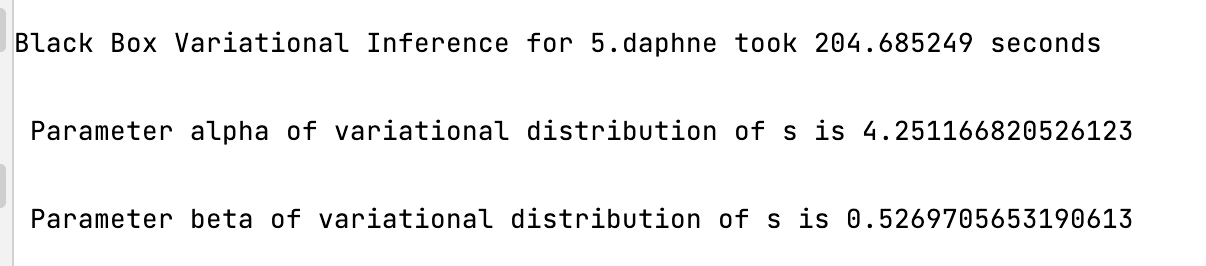
\includegraphics[scale=0.5]{../figs/5_daphne_results}
\end{figure}

\begin{figure}[!ht]
	\centering
	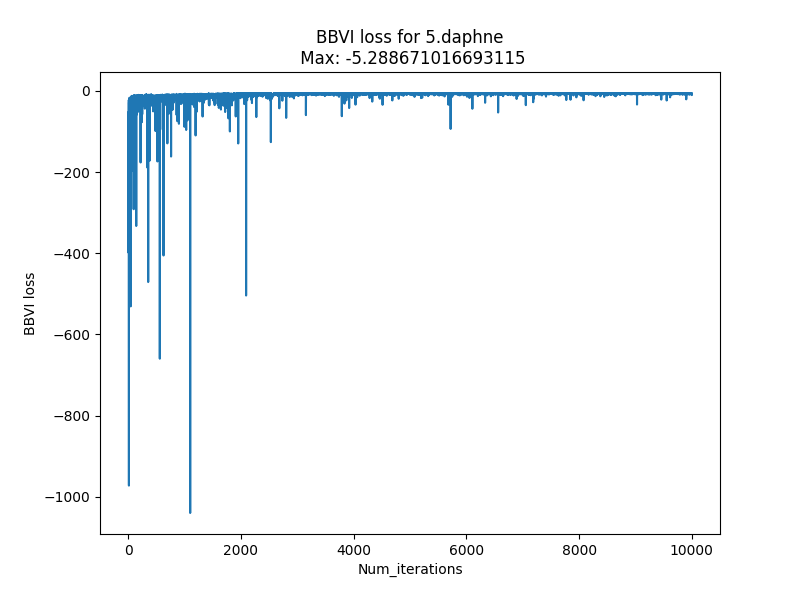
\includegraphics[scale=0.5]{../figs/5_daphne_ELBO}
\end{figure}

\begin{figure}[!ht]
	\centering
	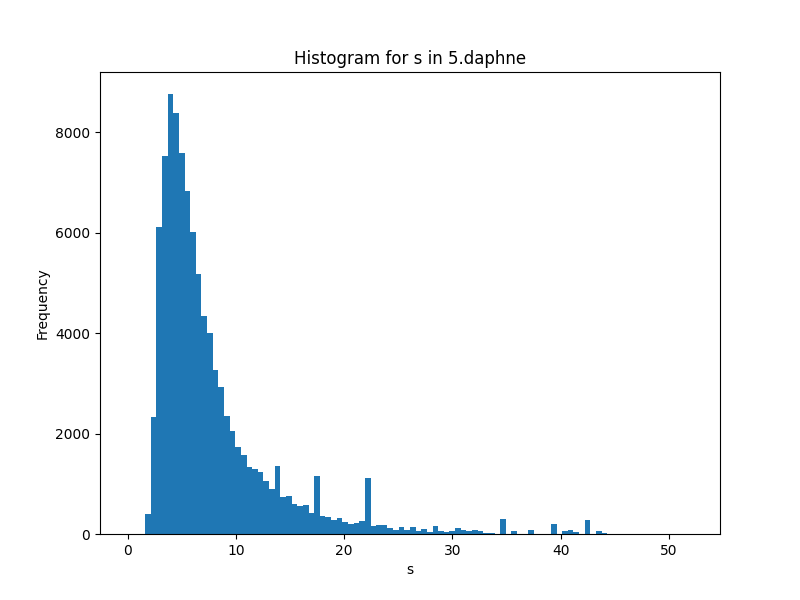
\includegraphics[scale=0.5]{../figs/5_daphne_s_histogram}
\end{figure}

\begin{figure}[!ht]
	\centering
	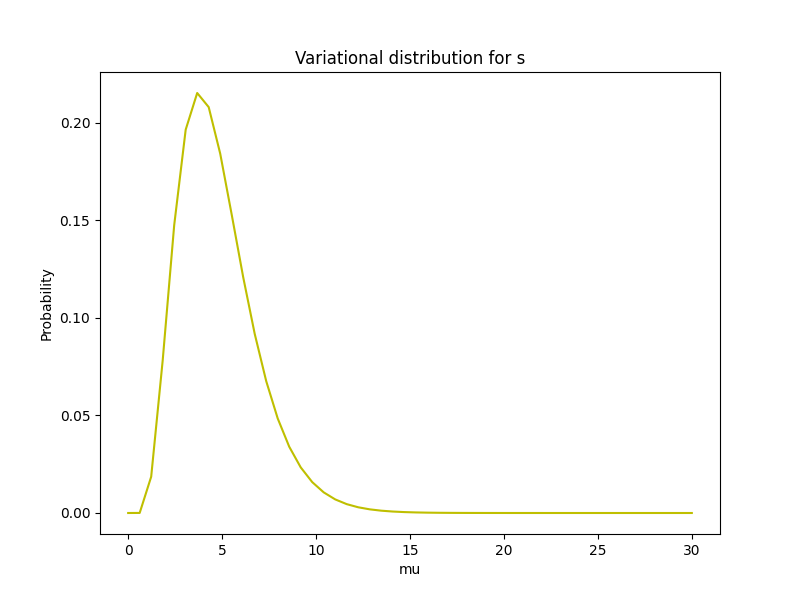
\includegraphics[scale=0.5]{../figs/5_daphne_pdf}
\end{figure}

\end{enumerate}
\end{document}